%
% LATEXBONES
%
\documentclass[a4paper,11pt,twoside]{article}
\usepackage{graphicx}
\usepackage{amsmath}
\usepackage[english]{babel}
\usepackage[applemac]{inputenc}
\usepackage[colorlinks,bookmarks=false,linkcolor=blue,urlcolor=blue]{hyperref}
\usepackage{subfigure}
\usepackage{here}
\usepackage{wrapfig}
\usepackage{fancyhdr}
\usepackage{dirtytalk}

%drow graph
\usepackage{fancybox}
\usepackage{tikz}
\usepackage{capt-of}

% print code
\usepackage{listings}
\usepackage{algorithm2e}
\usepackage{verbatim}

% push at the bottom
\newenvironment{bottompar}{\par\vspace*{\fill}}{\clearpage}

% landscape
\usepackage{pdflscape}

\paperheight=297mm
\paperwidth=210mm

\setlength{\textheight}{235mm}
\setlength{\topmargin}{-1.2cm} 

\setlength{\parindent}{0pt}

\setlength{\textwidth}{15cm}
\setlength{\oddsidemargin}{0.56cm}
\setlength{\evensidemargin}{0.56cm}

% quotes
\usepackage{framed}
\newcommand*{\signed}[1]{%
  \unskip\hspace*{1em plus 1fill}%
  \nolinebreak[3]\hspace*{\fill}\mbox{#1}
}

\pagestyle{plain}

% --- equations ---
\def \be {\begin{equation}}
\def \ee {\end{equation}}
%\def \dd  {{\rm d}}m

% --- links ---
\newcommand{\mail}[1]{{\href{mailto:#1}{#1}}}
\newcommand{\ftplink}[1]{{\href{ftp://#1}{#1}}}






% ======= Document ======

%----------------------------------------------------------------------------------------
% HEADING SECTIONS
%----------------------------------------------------------------------------------------

% --- header ---
\fancyhead[L]{Applied Data Analysis}
\fancyhead[R]{Summary}

\begin{document}
\begin{titlepage} %Titre
\begin{center}
\newcommand{\HRule}{\rule{\linewidth}{0.5mm}} % Defines a new command for the horizontal lines, change thickness here
\center % Center everything on the page
 
 
 %----------------------------------------------------------------------------------------
% TITLE SECTION
%----------------------------------------------------------------------------------------




\begin{figure} [h] %----------- SubGraph ---------------------
\centerline{
\subfigure{
\includegraphics[height = 2 cm]{./pic/EPFL.png}  }
\subfigure{
\includegraphics[height = 2 cm]{./pic/ADA-logo.png}} 
} 
\end{figure}


\vspace{0.5cm}
%\textsc{\LARGE EPFL}\\[1.5cm] % Name of your university/college
\textsc{\Large School Of Computer And Communication Sciences}\\[0.5cm] % Major heading such as course name
\textsc{\Large }\\% Minor heading such as course title
%\textsc{ \Large Master Semester Project}\\ % Minor heading such as course title


\HRule \\[0.4cm]
{ \huge \bfseries Applied Data Analysis \\Summary}\\[0.4cm] % Title of your document
\HRule \\[1.5cm]

% ---- Lovelace -----
\begin{center}
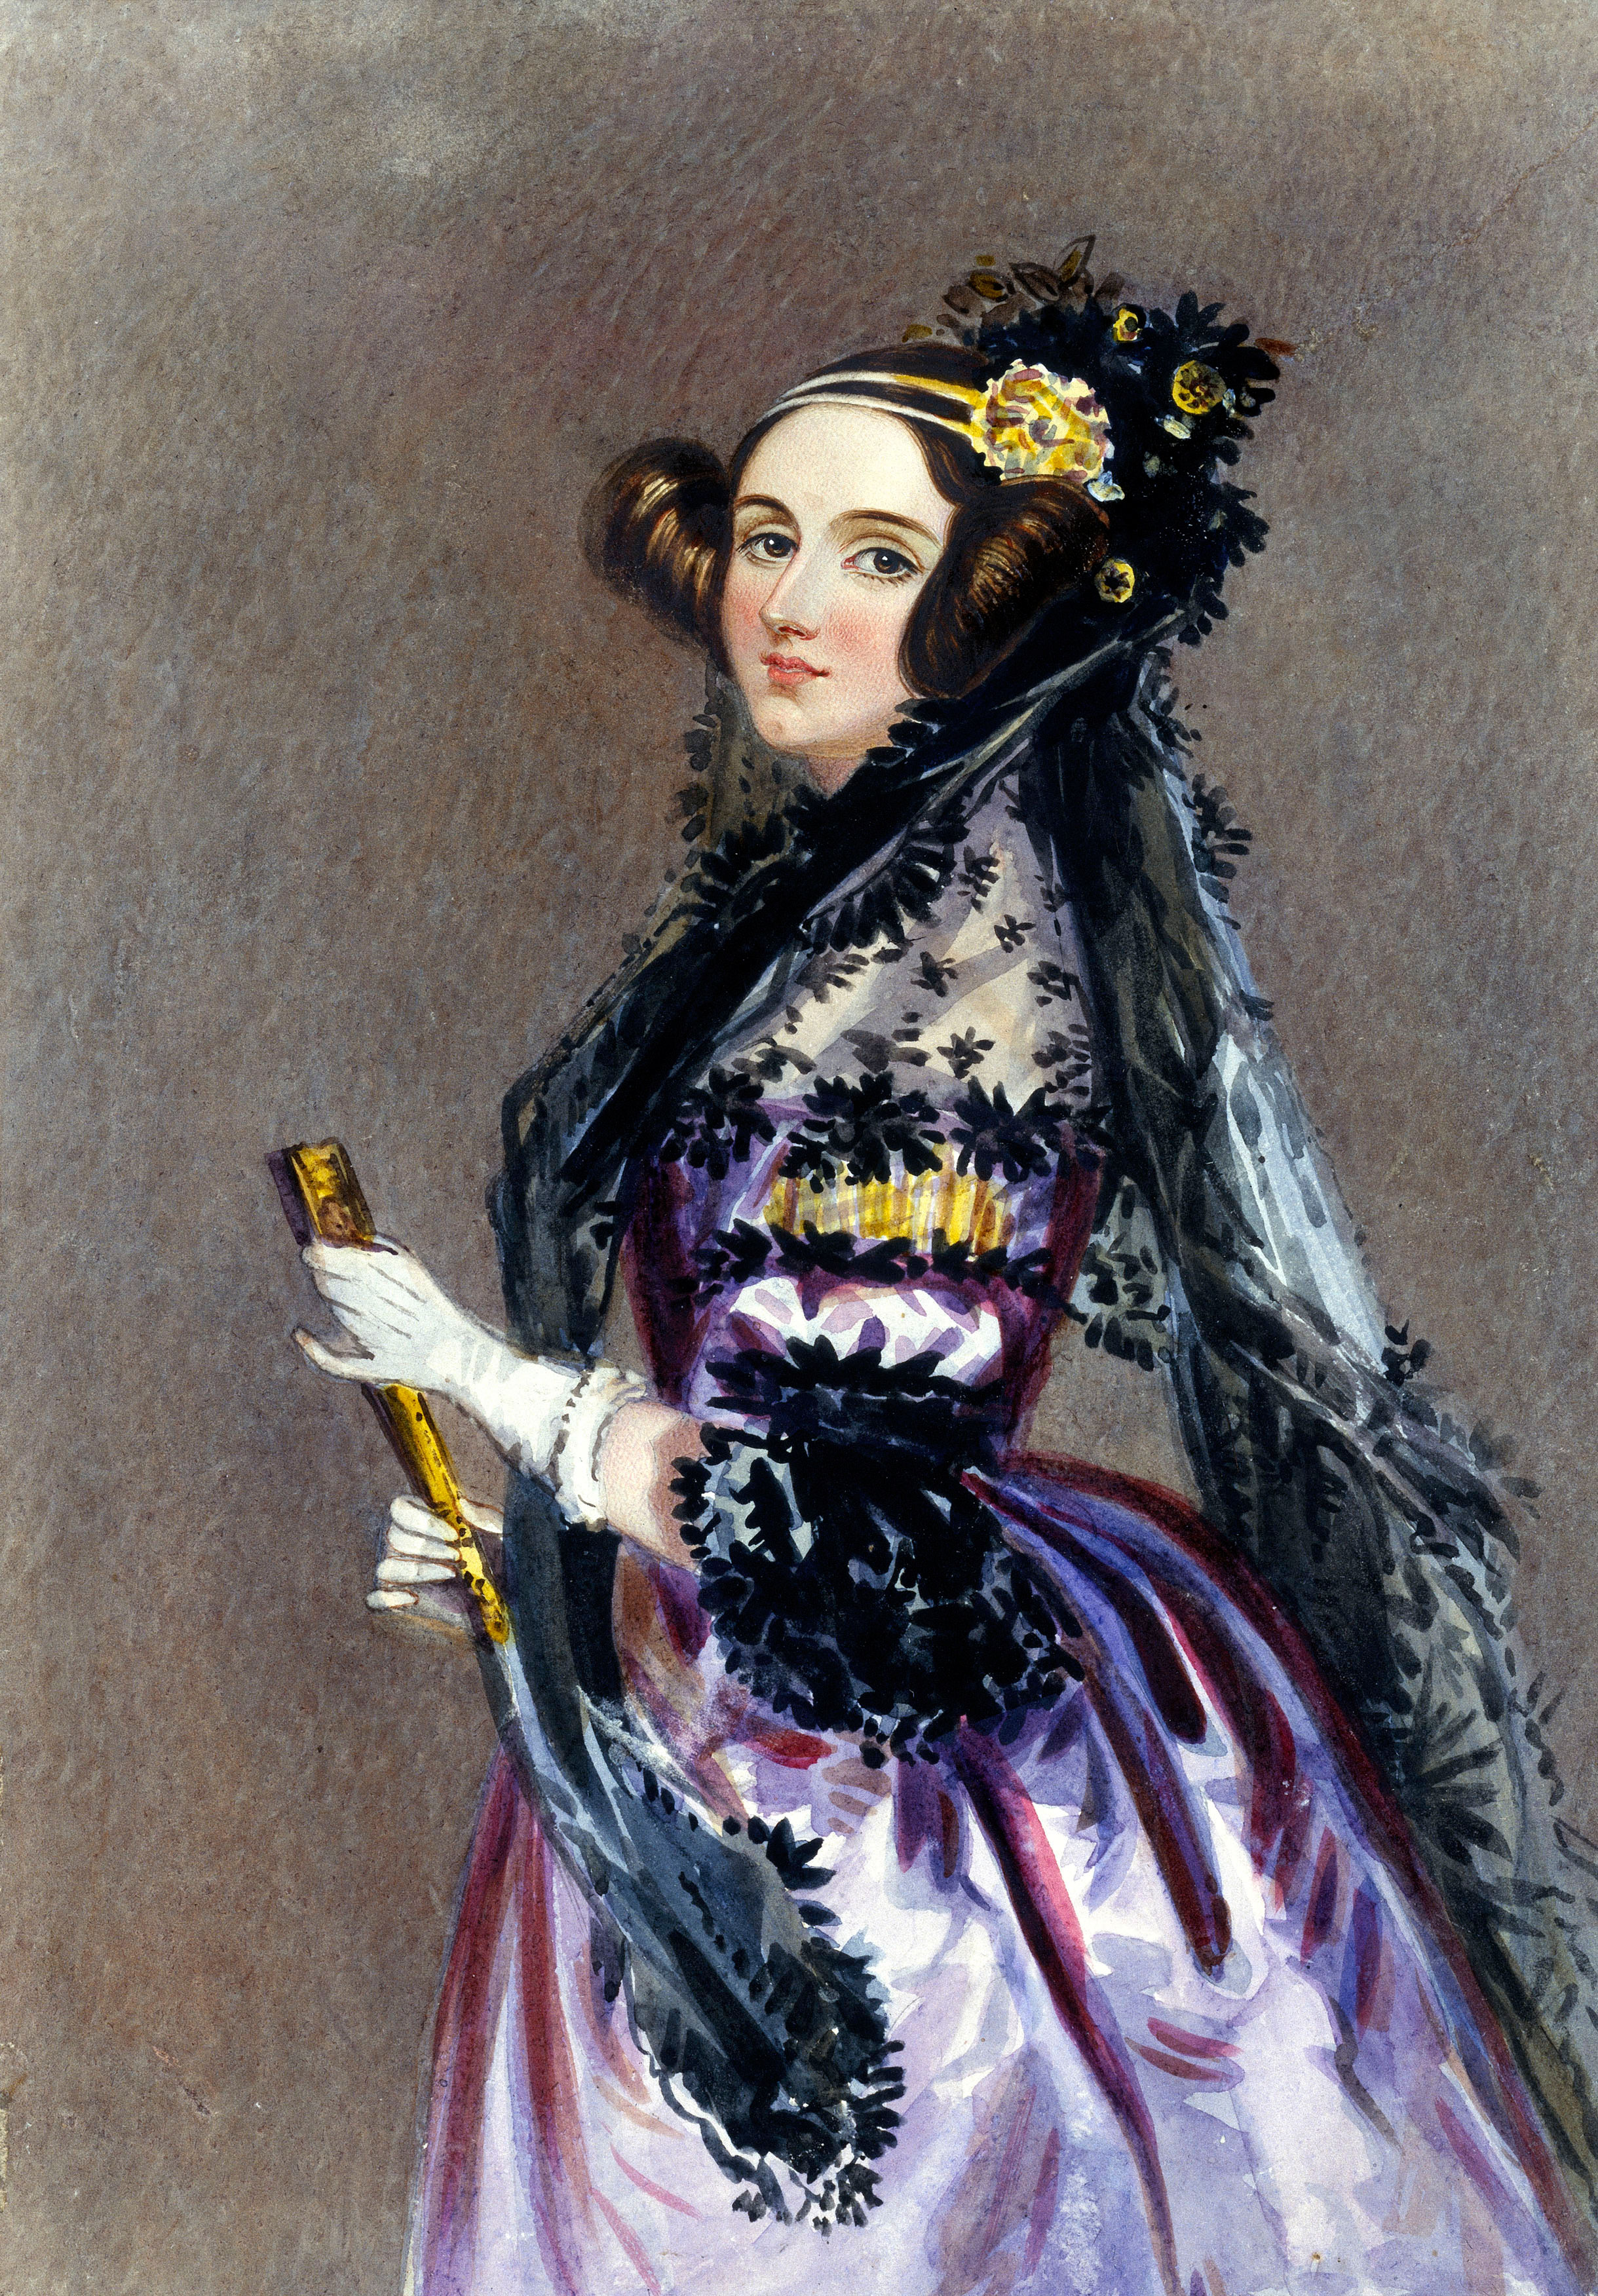
\includegraphics[width = 5 cm]{pic/lovelace} % Include a department/university logo - this will require the graphicx package
\end{center}



\begin{bottompar}
% ---- Professor -----
\begin{flushleft} \large
Prof. \textsc{Catasta} Michele\\
Distributed Information Systems Laboratory (LSIR) \\
\mail{michele.catasta@epfl.ch} \\ 
\end{flushleft}

% ---- date
{\large June 10, 2016}\\[1cm] % Date, change the \today to a set date if you want to be precise

\end{bottompar}
 
%%----------------------------------------------------------------------------------------
%% AUTHOR SECTION
%%----------------------------------------------------------------------------------------

%
%
%
%
%
%\begin{minipage}[t]{0.4\textwidth}
%
%\end{minipage}
%~
%\begin{minipage}[t]{0.55\textwidth}
%%\begin{flushright} \large
%%\emph{Assistant:} \\
%%\textsc{Voirol} Nicolas \\
%%PhD student\\
%%\mail{nicolas.voirol@epfl.ch} \\ [0.4cm]
%%
%%\emph{Supervisor:} \\
%%\textsc{Kuncak} Viktor\\  % Supervisor's Name
%%Professor\\
%%LARA - Laboratory for Automated Reasoning and Analysis\\
%%\mail{viktor.kuncak@epfl.ch}
%%\end{flushright}
%\end{minipage}\\[2cm]

% If you don't want a supervisor, uncomment the two lines below and remove the section above
%\Large \emph{Author:}\\
%John \textsc{Smith}\\[3cm] % Your name

%----------------------------------------------------------------------------------------
% LOGO SECTION
%----------------------------------------------------------------------------------------



%----------------------------------------------------------------------------------------
% DATE SECTION
%----------------------------------------------------------------------------------------

%{\Large \today}\\[1cm] % Date, change the \today to a set date if you want to be precise


%
%\begin{center}
%\abstract{\large Experiment various methods to compare functional trees between them. Given a function, use these algorithms to find the most similar tree contained in a corpus of functions. Try to suggest an autocompletion for a "hole" in a tree, based on this corpus.}
%\end{center} 
 %{\Large IDQ CONFIDENTIAL}
%----------------------------------------------------------------------------------------
\vfill % Fill the rest of the page with whitespace

\end{center}
\end{titlepage}



\pagestyle{fancy}
% ================ Table of content ==============
\newpage
\tableofcontents 

\baselineskip=16pt
%\parindent=15pt
%\parskip=5pt

\newpage




% ================ Introduction ==============
\section{Introduction}

\subsection{General information about the course}

This course covers multiple topics in the data science field such as \textbf{Data Wrangling}, {\bf Data Management}, {\bf Data Mining}, {\bf Machine Learning}, {\bf Visualization}, {\bf Statistics} and {\bf Story telling}. It's about {\bf breadth}, not depth. Indeed, Data science is evolving really quickly, hence learning in depth a specific tool won't pay off. 

\subsection{Data Science}

When we talk about Data Science, we often use the term Big Data as the enormous amount of data that exist in the world. But Big Data is not only about collecting huge amount of data. It is challenging but not enough. The real value comes from the insights. The {\it internet} companies (Google, Facebook, etc.) 
understood this many years ago.
\\ \\
An accurate definition of Data Analysis is given by Wikipedia:
\begin{framed}
{\it {\bf Analysis of data} is a process of {\bf inspecting}, {\bf cleaning}, {\bf transforming}, and {\bf modeling data} with the goal of {\bf discovering useful information}, suggesting conclusions, and supporting decision-making.
Data analysis has multiple facets and approaches, encompassing diverse techniques under a variety of names, {\bf in different business}, science, and social science {\bf domains}.}
\signed{\href{https://en.wikipedia.org/wiki/Data\_analysis}{Wikipedia - Data Analysis}}
\end{framed}

Therefore, a Data Scientist has to master different kind of skills such as {\bf Mathematics} (for the Statistics), {\bf Programming} and the {\bf Domain Expertise}. Drew Conway's Venn diagram, Figure \ref{img:venn}, shows the different combination man can obtain with these three skills.

\begin{figure}[H]
 \centering
 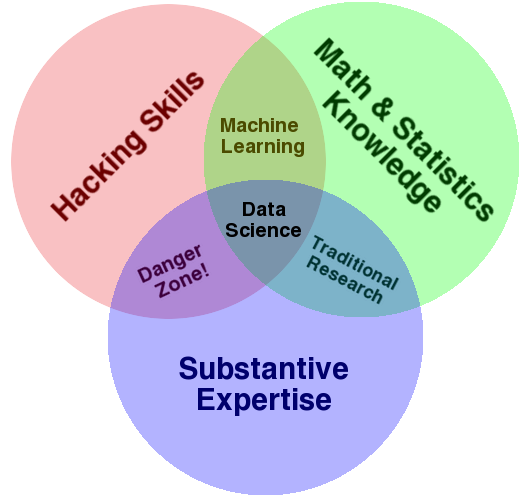
\includegraphics[width=7cm]{./pic/Data_Science_VD.png}
 \caption{\label{img:venn} Venn Diagram describing the different combination of skills used by a Data Scientist (by Drew Conway)}
\end{figure}

\begin{figure}[H]
 \centering
 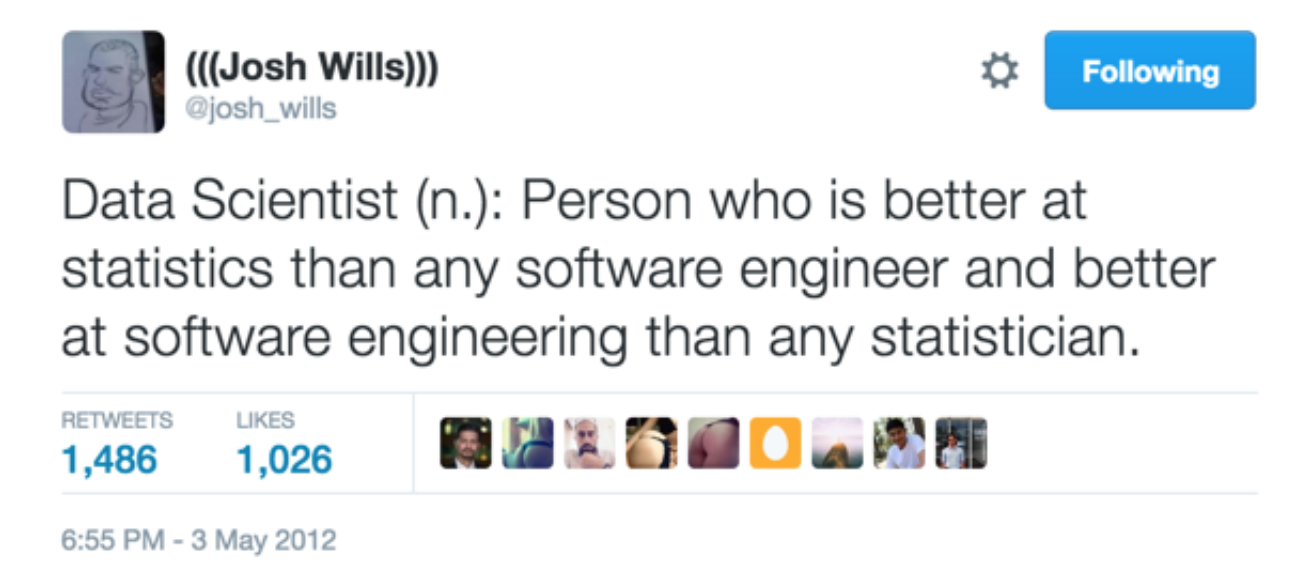
\includegraphics[width=10cm]{./pic/tweet_wills.png}
 \caption{\label{img:tweet_wills} A tweet from Josh Wills, Data Scientist at Slack.}
\end{figure}

{\bf A practical definition of Data Science} 

Data Science is about the whole processing pipeline to extract information out of data. As such, a Data Scientist {\bf understands and cares about the whole data pipeline}.

\begin{minipage}{0.5\textwidth}
\begin{figure}[H]
 \centering
 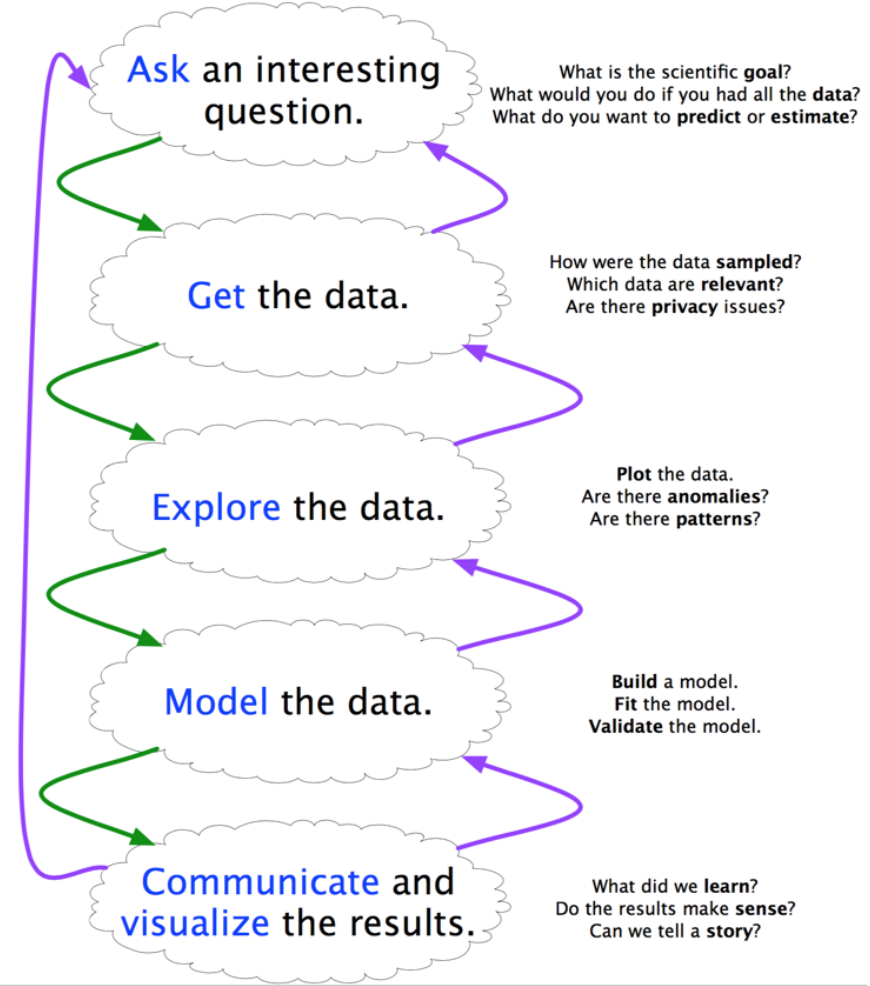
\includegraphics[width=8cm]{./pic/pipeline.png}
\end{figure}
\end{minipage} \hfill
\begin{minipage}{0.45\textwidth}
A {\bf data pipeline} consists of 3 steps:
\begin{enumerate}
 \item Preparing to run a model. \\
  {\it Gathering, cleaning, integrating, restructuring, transforming, loading, filtering, deleting, combining, merging, verifying, extracting, shaping}
 \item Running the model
 \item Communicating the results
\end{enumerate}
\vspace{0.5cm}
 A ``good'' Data Scientist will always go back and forth between the steps. The diagram on the left shows exactly what can happen. 
\end{minipage}
\\ \\
In this course, you will develop the following skills:
\begin{description}
 \item[data muning/scraping/sampling/cleaning] in order to get an informative, manageable data setlength
 \item[data storage and management] in order to be able to access data quickly and reliably during subsequent analysis
 \item[exploratory data analysis] to generate hypotheses and intuition about the data
 \item[prediction] based on statistical tools such as regression, classification, and clustering
 \item[communication of results] through visualization, stories and interpretable summaries
\end{description}

\section{Data Wrangling}







%======= TABLEAU ===========
%\begin{center} %---------------Tab--------------
%\begin{tabular} {| c | c | c | c | c | c |}
%\hline
 %& & & & & $\\ \hline
%\end{tabular}
%\end{center}


%===========GRAPH================
%\begin{figure} %---------------------Graph---------------------------
%\begin{center}
%\includegraphics[width=12cm]{graph/ampli2} 
%\end{center}
%\caption{\em  \label{label}
%L�gende
%}
%\end{figure}


%========SUBGRAPH=======
%\begin{figure} [h] %----------- SubGraph ---------------------
%\centerline{
%\subfigure[ sublegend ] {\label{sfig:thetat} \includegraphics[width=7cm]{ graph/graph_convdt3 } }
%\subfigure[ sublegend ] {\label{sfig:thetafin} \includegraphics[width=7cm]{ graph/graph_convtfin } } 
%}
%\caption{\label{ label } 
%L�gende
%} 
%\end{figure}








\end{document} %%%% THE END %%%%
